\documentclass[
%% TIKZ_CLASSOPTION %%
tikz
]{standalone}
\usepackage{amsmath}
\usetikzlibrary{matrix}
%% EXTRA_TIKZ_PREAMBLE_CODE %%
\begin{document}
%% TIKZ_CODE %%
\usetikzlibrary{positioning}
\usetikzlibrary{shapes.geometric}
\usetikzlibrary{arrows}
\usetikzlibrary{decorations}
\tikzstyle{Arrow} = [->, thin, preaction = {decorate}]
\tikzset{>=latex}

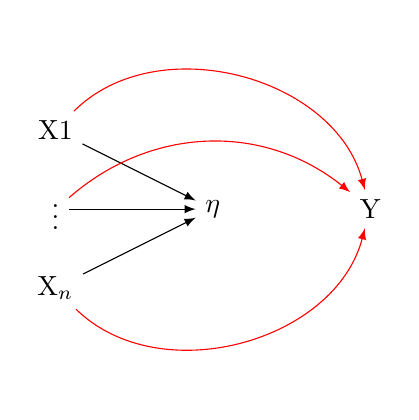
\begin{tikzpicture}[{every node/.append style}=draw]


%\node [draw=white] (L) at (0, 0) {L};
\node [rectangle, draw=white] (X1) at (2, 1) {X1};
\node [rectangle, draw=white] (X2) at (2, 0) {$\vdots$};
\node [rectangle, draw=white] (Xn) at (2, -1) {X$_n$};
\node [rectangle, draw=white] (eta) at (4, 0) {$\eta$};
\node [rectangle, draw=white] (Y) at (6, 0) {Y};



\draw [-latex, draw=black] (X1) to (eta);
\draw [-latex, draw=black] (X2) to (eta);
\draw [-latex, draw=black] (Xn) to (eta);
%\draw [-latex, bend left=80, draw=black] (L) to (Y);
\draw [-latex, bend left=60, draw=red] (X1) to (Y);
\draw [-latex, bend left=40, draw=red] (X2) to (Y);
\draw [-latex, bend right =60,  draw=red] (Xn) to (Y);



\end{tikzpicture}
\end{document}
